\section{Introduction}
\label{sec:intro}

Coding agents combine language-model reasoning with a shell, a filesystem, and the ability to
write and execute programs. These capabilities could also support tasks whose goal is not
software development: diagnosing a rare disease, formulating an optimization problem, finding
evidence in a large corpus, or analyzing scientific data. Domain-specific systems address these
tasks through specialized retrieval, tools, memory, and workflows. When does a general coding
agent rival those systems, and when does domain-specific structure still help?

We study this question using Codex on a suite of \StudyBenchmarkCount{} non-coding benchmarks selected from
554 candidate benchmark records. The collection spans 33 overlapping domain labels and includes
an 83-entry evidence shortlist and a 30-task feasibility-review inventory, each subject to
further selection. SSTQA replaces LongBench v2 in the study suite because the selected DeLM
implementation for LongBench v2 is unavailable; the earlier LongBench measurement remains
in the supplementary results. We incorporate the available reruns and distinguish primary
settings from scored variants throughout. The resulting
suite covers clinical and biomedical reasoning, chemistry and materials science, operations
research, financial and tabular reasoning, retrieval, long-context aggregation, and scientific
research. This breadth makes it possible to examine differences across task types rather than
treat generalization beyond coding as a single score.

\begin{figure}[t]
  \centering
  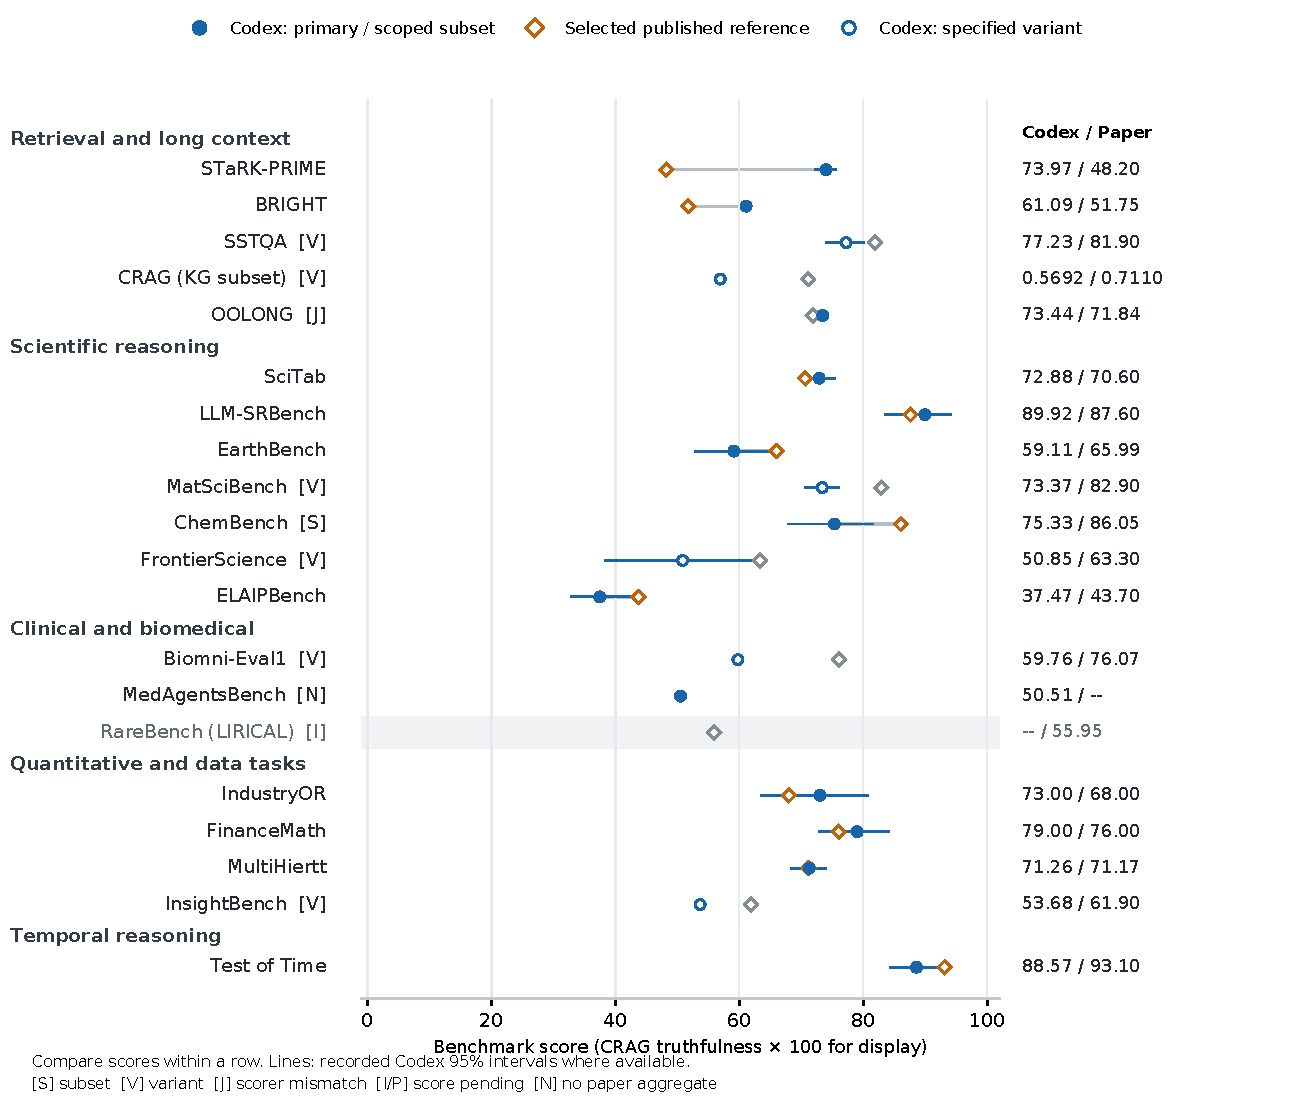
\includegraphics[width=\textwidth]{figures/direct_codex_vs_published.pdf}
  \caption{Direct Codex and selected published reference scores after the HF result refresh.
  Filled circles show primary settings or declared planned subsets; open circles show scored
  protocol variants. ChemBench uses a 150-question open-web pilot; SSTQA shows the English-split
  judge variant, with its Chinese-split primary result pending. RareBench awaits a valid
  network-enabled run. Each row uses its own
  metric (CRAG truthfulness is multiplied by 100 for plotting).
  Appendix~\ref{app:result-details} records coverage, variants, and score provenance. Lines between
  systems mark descriptive paper comparisons, which include backbone and protocol differences.}
  \label{fig:main-results}
\end{figure}

\paragraph{Two complementary comparisons.}
Figure~\ref{fig:main-results} gives the broad comparison with scores reported in the literature.
It answers how the measured coding agent relates to existing reported performance, while retaining
each reference's model and evaluation setting. To examine the contribution of a scaffold, we also
execute specialized systems on a shared backbone and score both arms on the same instances.
These comparisons answer different questions: a gain over a published score may reflect a
stronger backbone, while a shared-backbone comparison more directly tests the system around it.
Reasoning effort, tool permissions, evaluator, and dataset version must still be checked.

\paragraph{A reusable benchmark audit pipeline.}
Establishing either comparison requires identifying the correct reference system, tracing its
score to a primary source, and translating its evaluation protocol into executable tasks.
Our AI-assisted pipeline records these steps as benchmark specifications, run contracts,
declared patches, and auditable evidence (Figure~\ref{fig:audit-pipeline}). It also exposes
limitations of the available benchmark ecosystem: unavailable resources, ambiguous metrics,
changes in answer keys, and differences between a released implementation and its reported
system. These are findings about evaluation design and reproducibility. They are kept separate
from explanations of why one agent solves a task better than another.

\paragraph{Contributions.}
We contribute (1) a broad audit of 554 candidate benchmark records and an evaluation
suite supporting a study covering \StudyBenchmarkCount{} non-coding benchmarks; (2) a reusable pipeline for
finding published reference systems, validating executable evaluations, and documenting the
conditions of comparison; and (3) an empirical comparison organized around experimental rigor,
domain-level performance differences, and the mechanisms behind successes and failures.
Available measurements are included in this draft. The 25\%-subset comparator campaign and
the remaining paired trace analyses are in progress, with unfinished results explicitly marked.

The study evaluates one Codex configuration, not the population of coding agents. Its benchmark
collection is a documented, AI-assisted meta-analysis rather than an exhaustive systematic
review, and its heterogeneous metrics are not pooled into a single performance average.
